\chapter{Results}
\label{chap:results}

\drop{T}{he} obtained results of the implementation, execution and
validation of the GEO-Cloud experiment are explained. The \emph{PlanetLab}
experiment for measuring the network impairments (bandwidth, loss-rate and
\ac{RTT}) are shown and plotted. These plots represents how the impairments
directly depends on the distance between both source and destination elements.
The next section shows the results of the execution of some defined scenarios into
the GEO-Cloud experiment. Finally, the evaluation of the implementation for processing
\ac{EO} images on-cloud is explained.


\section{PlanetLab Experiment Results}
\label{sec:pl-res}
During the execution of the \pl experiment (see Section~\ref{sec:planetlab}) 21600 communications were established between every node representing ground stations and users and the central node representing the cloud. The bandwidth, latency and loss rate were measured.
In Figure~\ref{fig:Bandwidth_gs_hist} the 21600 samples acquired in the communication between the node 22 and the central node during 6 hours of continuous execution are represented in a normalized histogram. The data accurately fits to a gaussian distribution with mean $3.28~Mbps$ and standard deviation $0.446~Mbps$. In Figure~\ref{fig:Latency_gs_hist} a normalized histogram of the measured latency is represented. It was fitted with a gaussian distribution with mean $154.210~ms$ and standard deviation $1.314~ms$. The loss rate between this node and the central node was obtained to be $0.0096$\%~\cite{Gonzalez2014}.
\begin{figure*}
\begin{center}
  \subfloat[Bandwidth of the node representing Chetumal ground station]{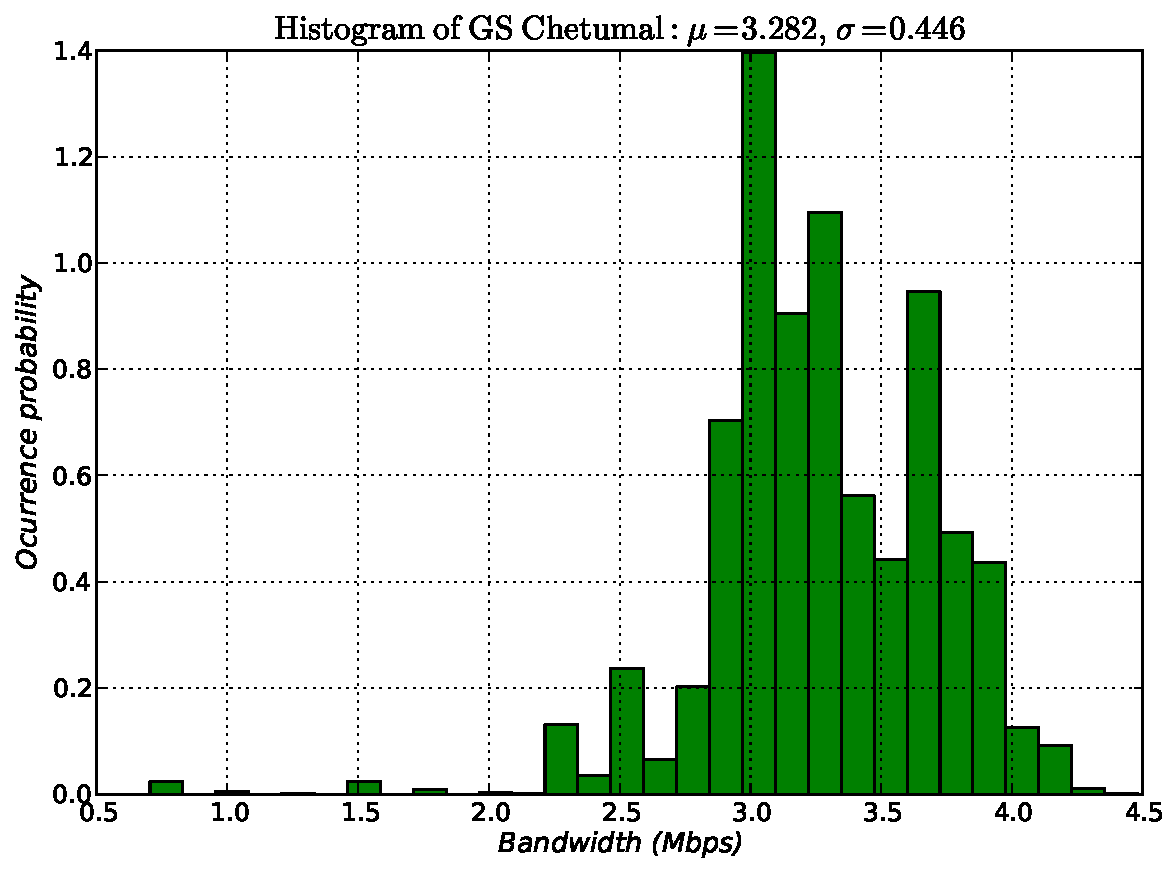
\includegraphics[scale=0.35]{resultsPL/IndividuallyGSHistChetumal.pdf}
 \label{fig:Bandwidth_gs_hist}}
\hspace{0.01\textwidth}
\subfloat[Latency of the node representing Chetumal ground
station]{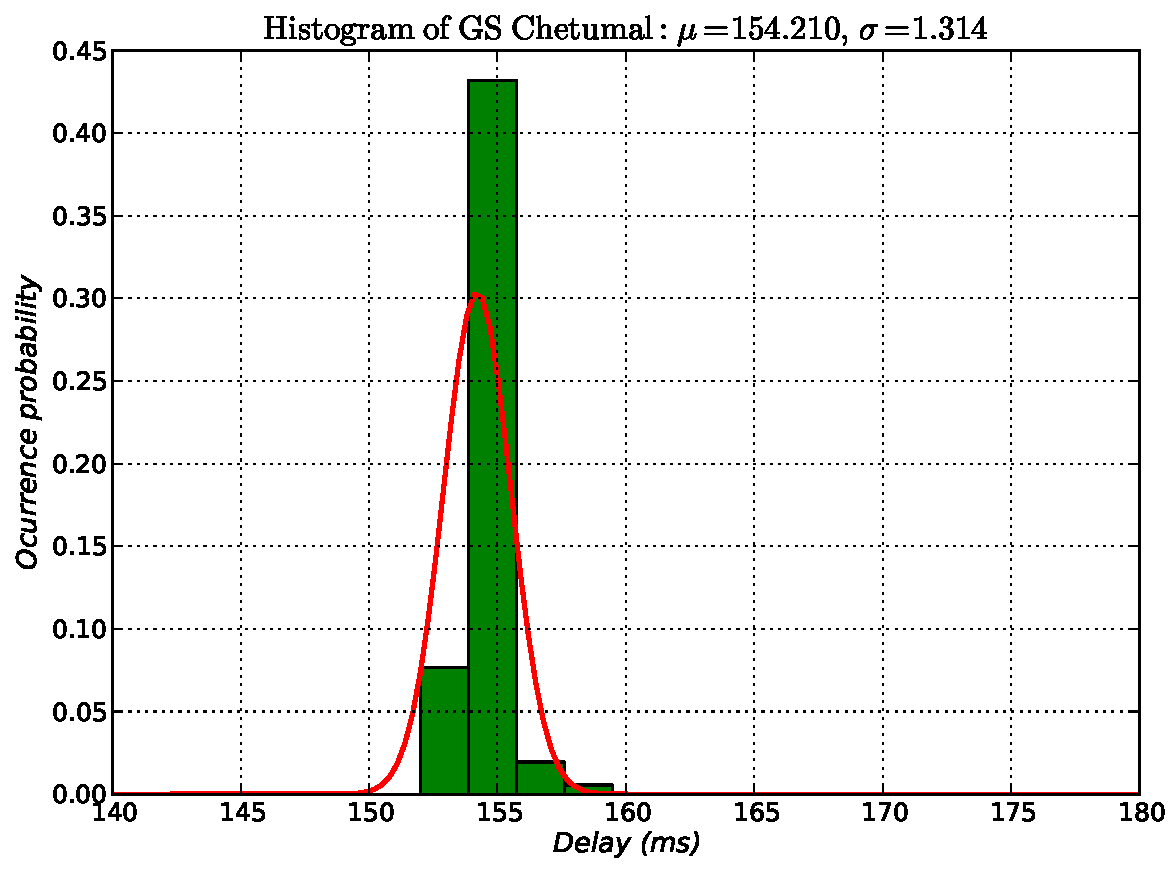
\includegraphics[scale=0.35]{resultsPL/DelayHistGSChetumal.pdf}
 \label{fig:Latency_gs_hist}}
\end{center}
\end{figure*}



The previous procedure was followed for the rest of the nodes. In
Figure~\ref{fig:bandwidth-plot} the mean and the standard deviation for each
node are depicted respectively. It can be observed that in general, the
bandwidth decreases when the distance between nodes increases. However the node
5 in Madrid presents a higher dispersion in the bandwidth value with respect to
the rest of nodes. It has a bandwidth of $15.2~Mbps$. The measurements were
fitted with different functions by using the least squares optimization
method. Exponential, polynomial, logarithm and hyperbolic functions were used to
fit the samples. For each fitted function the $R^2$ coefficient of
determination, which varies between 0 and 1, and indicates how well the
statistical distribution is fitted. The highest the value of the $R^2$, the
better the fitting. The following results were obtained: for exponential
function: $Bandwidth=4.655e^{-10^{-4}x}$,$R^2=0.5454$; for polynomial function
$Bandwidth=-3\cdot10^{-4}x+4.9444$, $R^2=0.3628$ and for logarithm function $Bandwidth=-1.519Ln(x)+15.325$, $R^2=0.4539$, where $x$ is the distance between any node and the central node in $km$. The bandwidth was obtained in $Mbps$. However, the hyperbolic function was the one that best fitted the distribution:
\begin{equation}\label{eq:bandwidth_fitting}
Bandwidth=184.91x^{-0.547};~R^2=0.582
\end{equation}

\begin{center}
\begin{figure}[h]
  \centering
  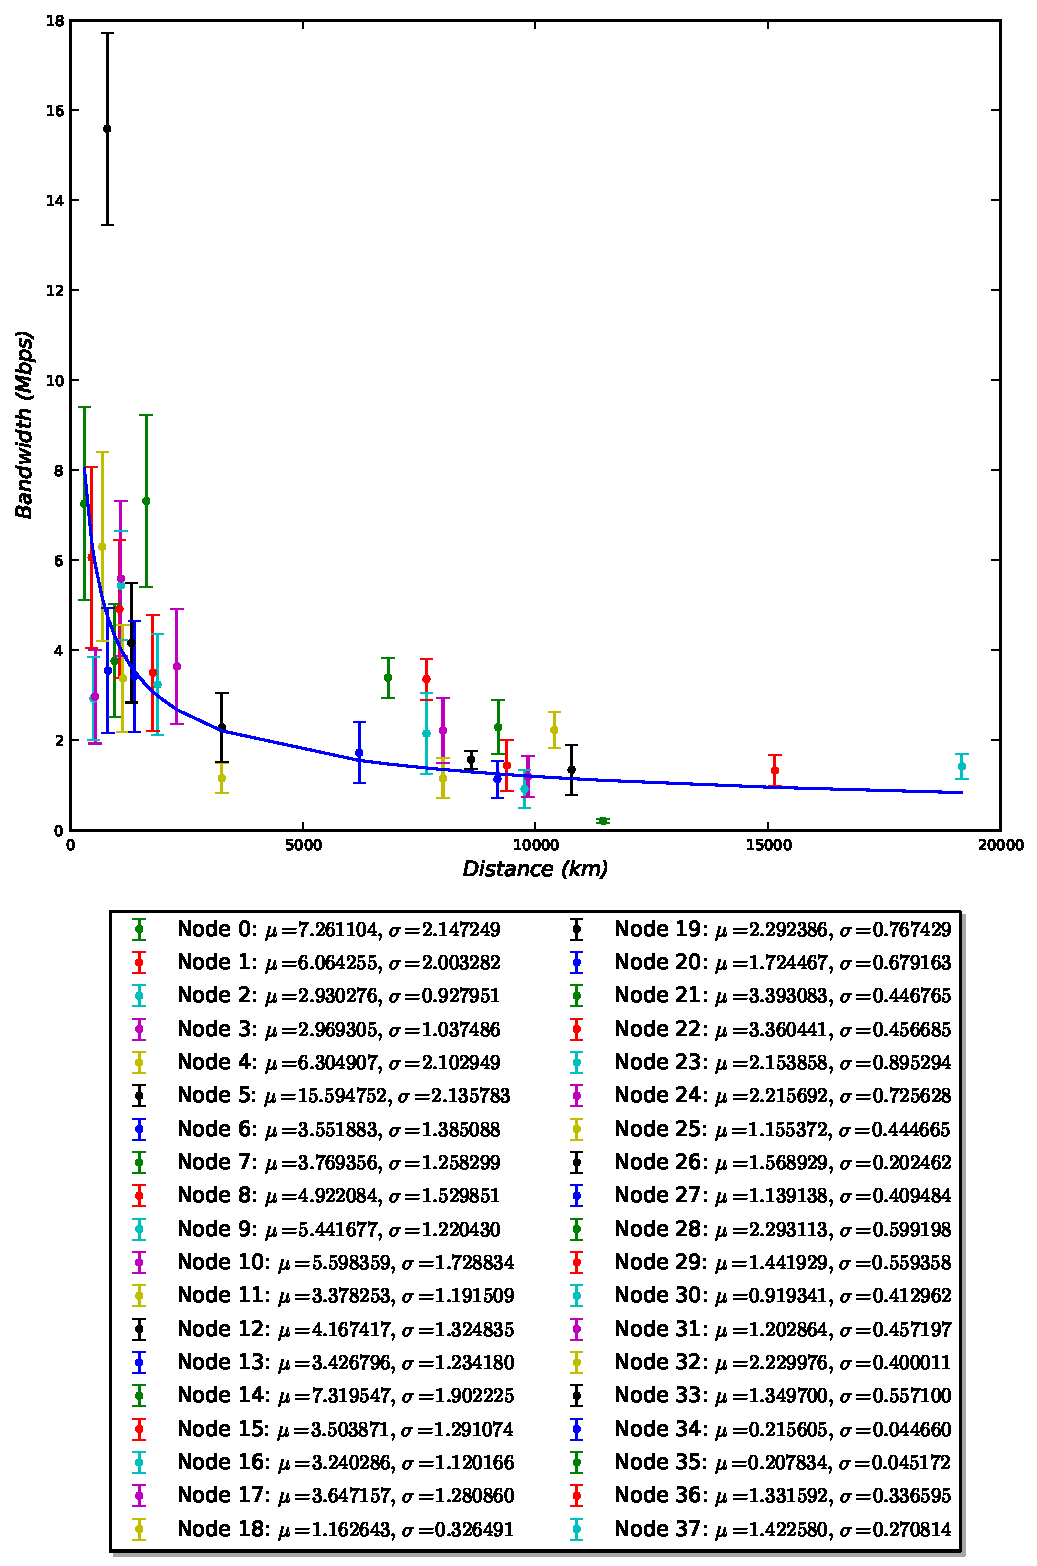
\includegraphics[scale=0.7]{resultsPL/bandwidthall.pdf}\\
  \caption{Bandwidth of all nodes} \label{fig:bandwidth-plot}
\end{figure}
\end{center}

Figure~\ref{fig:delay-plot} shows the mean and standard
deviation of the latency measured in all the nodes connecting the central node
in France. In this case the fitting used was a linear function. It accurately fitted the data distribution. The equation that approximated the data is the following:
\begin{equation}\label{eq:latency_fitting}
Latency=0.0228x+17.88;~R^2=0.8927
\end{equation}
The latency is obtained in $ms$ when the distance $x$ is introduced in $km$.


\begin{center}
\begin{figure}[h]
  \centering
  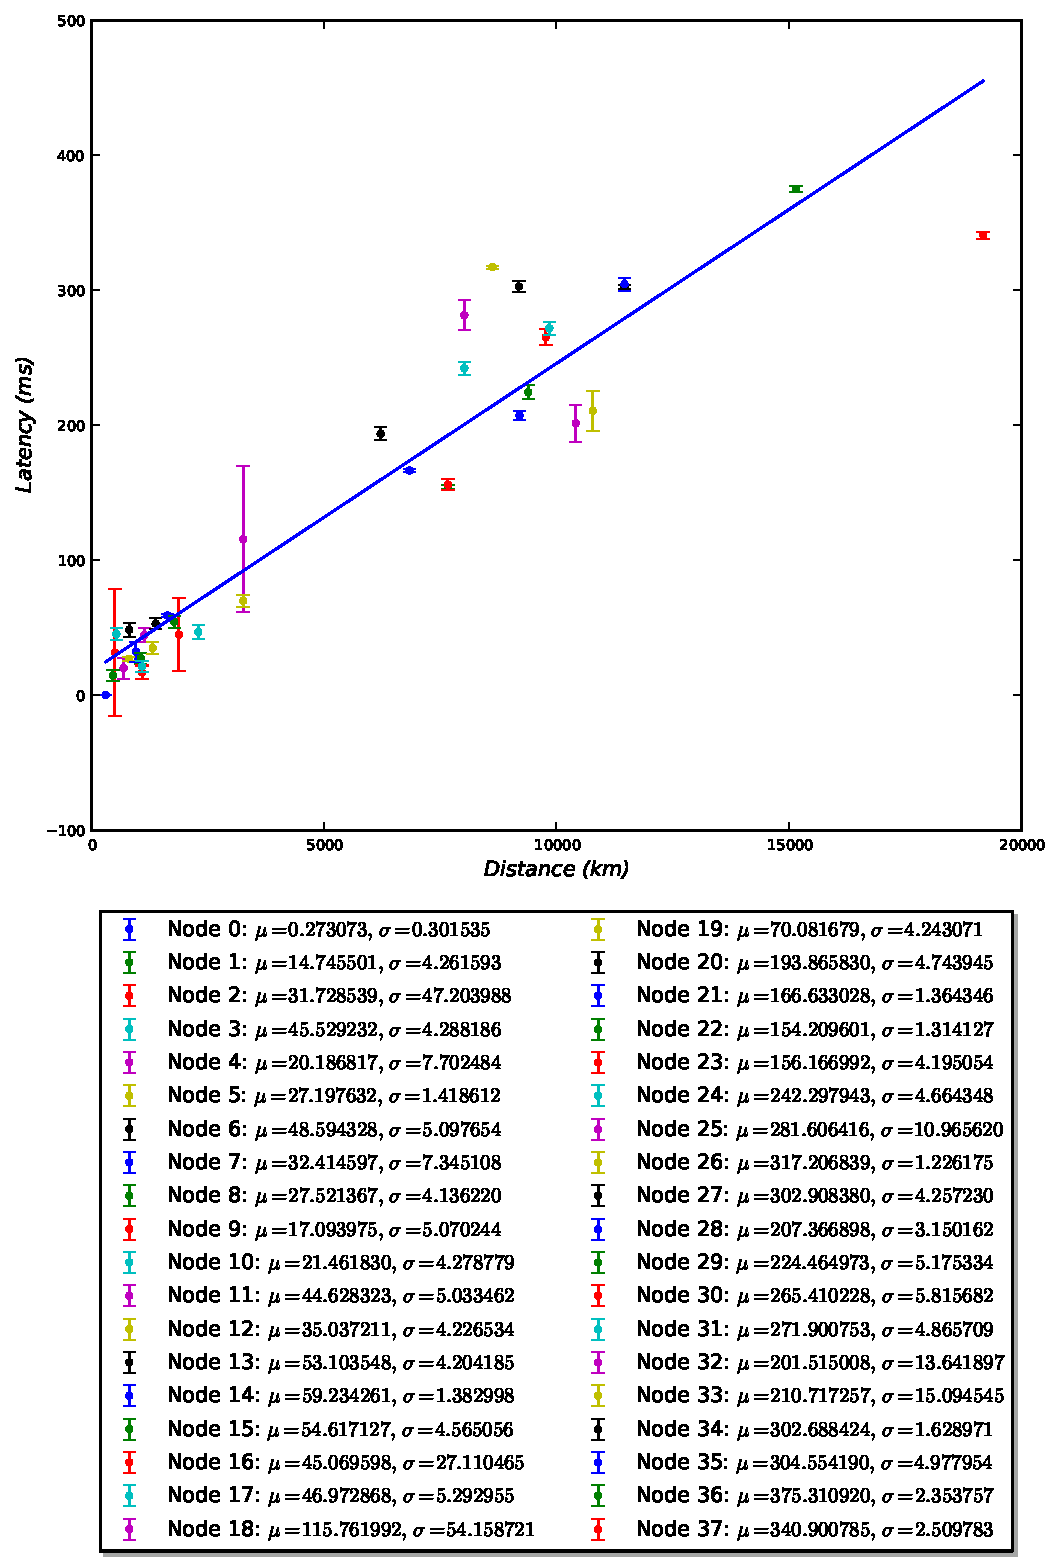
\includegraphics[scale=0.7]{resultsPL/DelayNodes.pdf}\\
  \caption{Latency of all nodes} \label{fig:delay-plot}
\end{figure}
\end{center}

Figure~\ref{fig:loss-rate-plot} shows the loss rate between any node and the central node during the whole execution of the experiment. In most of the communications the loss rate was under 0.2\%. Two cases are remarkable: on the one hand, between the node 20 in Russia and the central node 0\% of loss rate was measured, which means that no packets were lost; on the other hand, between Greece (node 16) and the central node, a loss rate of 15.68\% was measured, maybe because of interruptions in the network, overload of the server in Greece or routed network fails. The mean of the loss rates between all the communications was 0.053\% with a standard deviation of 0.097\% without considering the node in Greece in the calculations.

Table~\ref{anex:nodes-pl-results} summarizes the obtained measures. Column 5 and 6 show the mean and
the standard deviation of the bandwidth measured in all the nodes connecting the
central node in France. Column 7 and 8 also depict the mean and standard
deviation of the latency in the nodes. Finally, column 9 represents the measured
loss-rate between any node and the central node during the experiment.




\begin{center}
\begin{figure}[h]
  \centering
  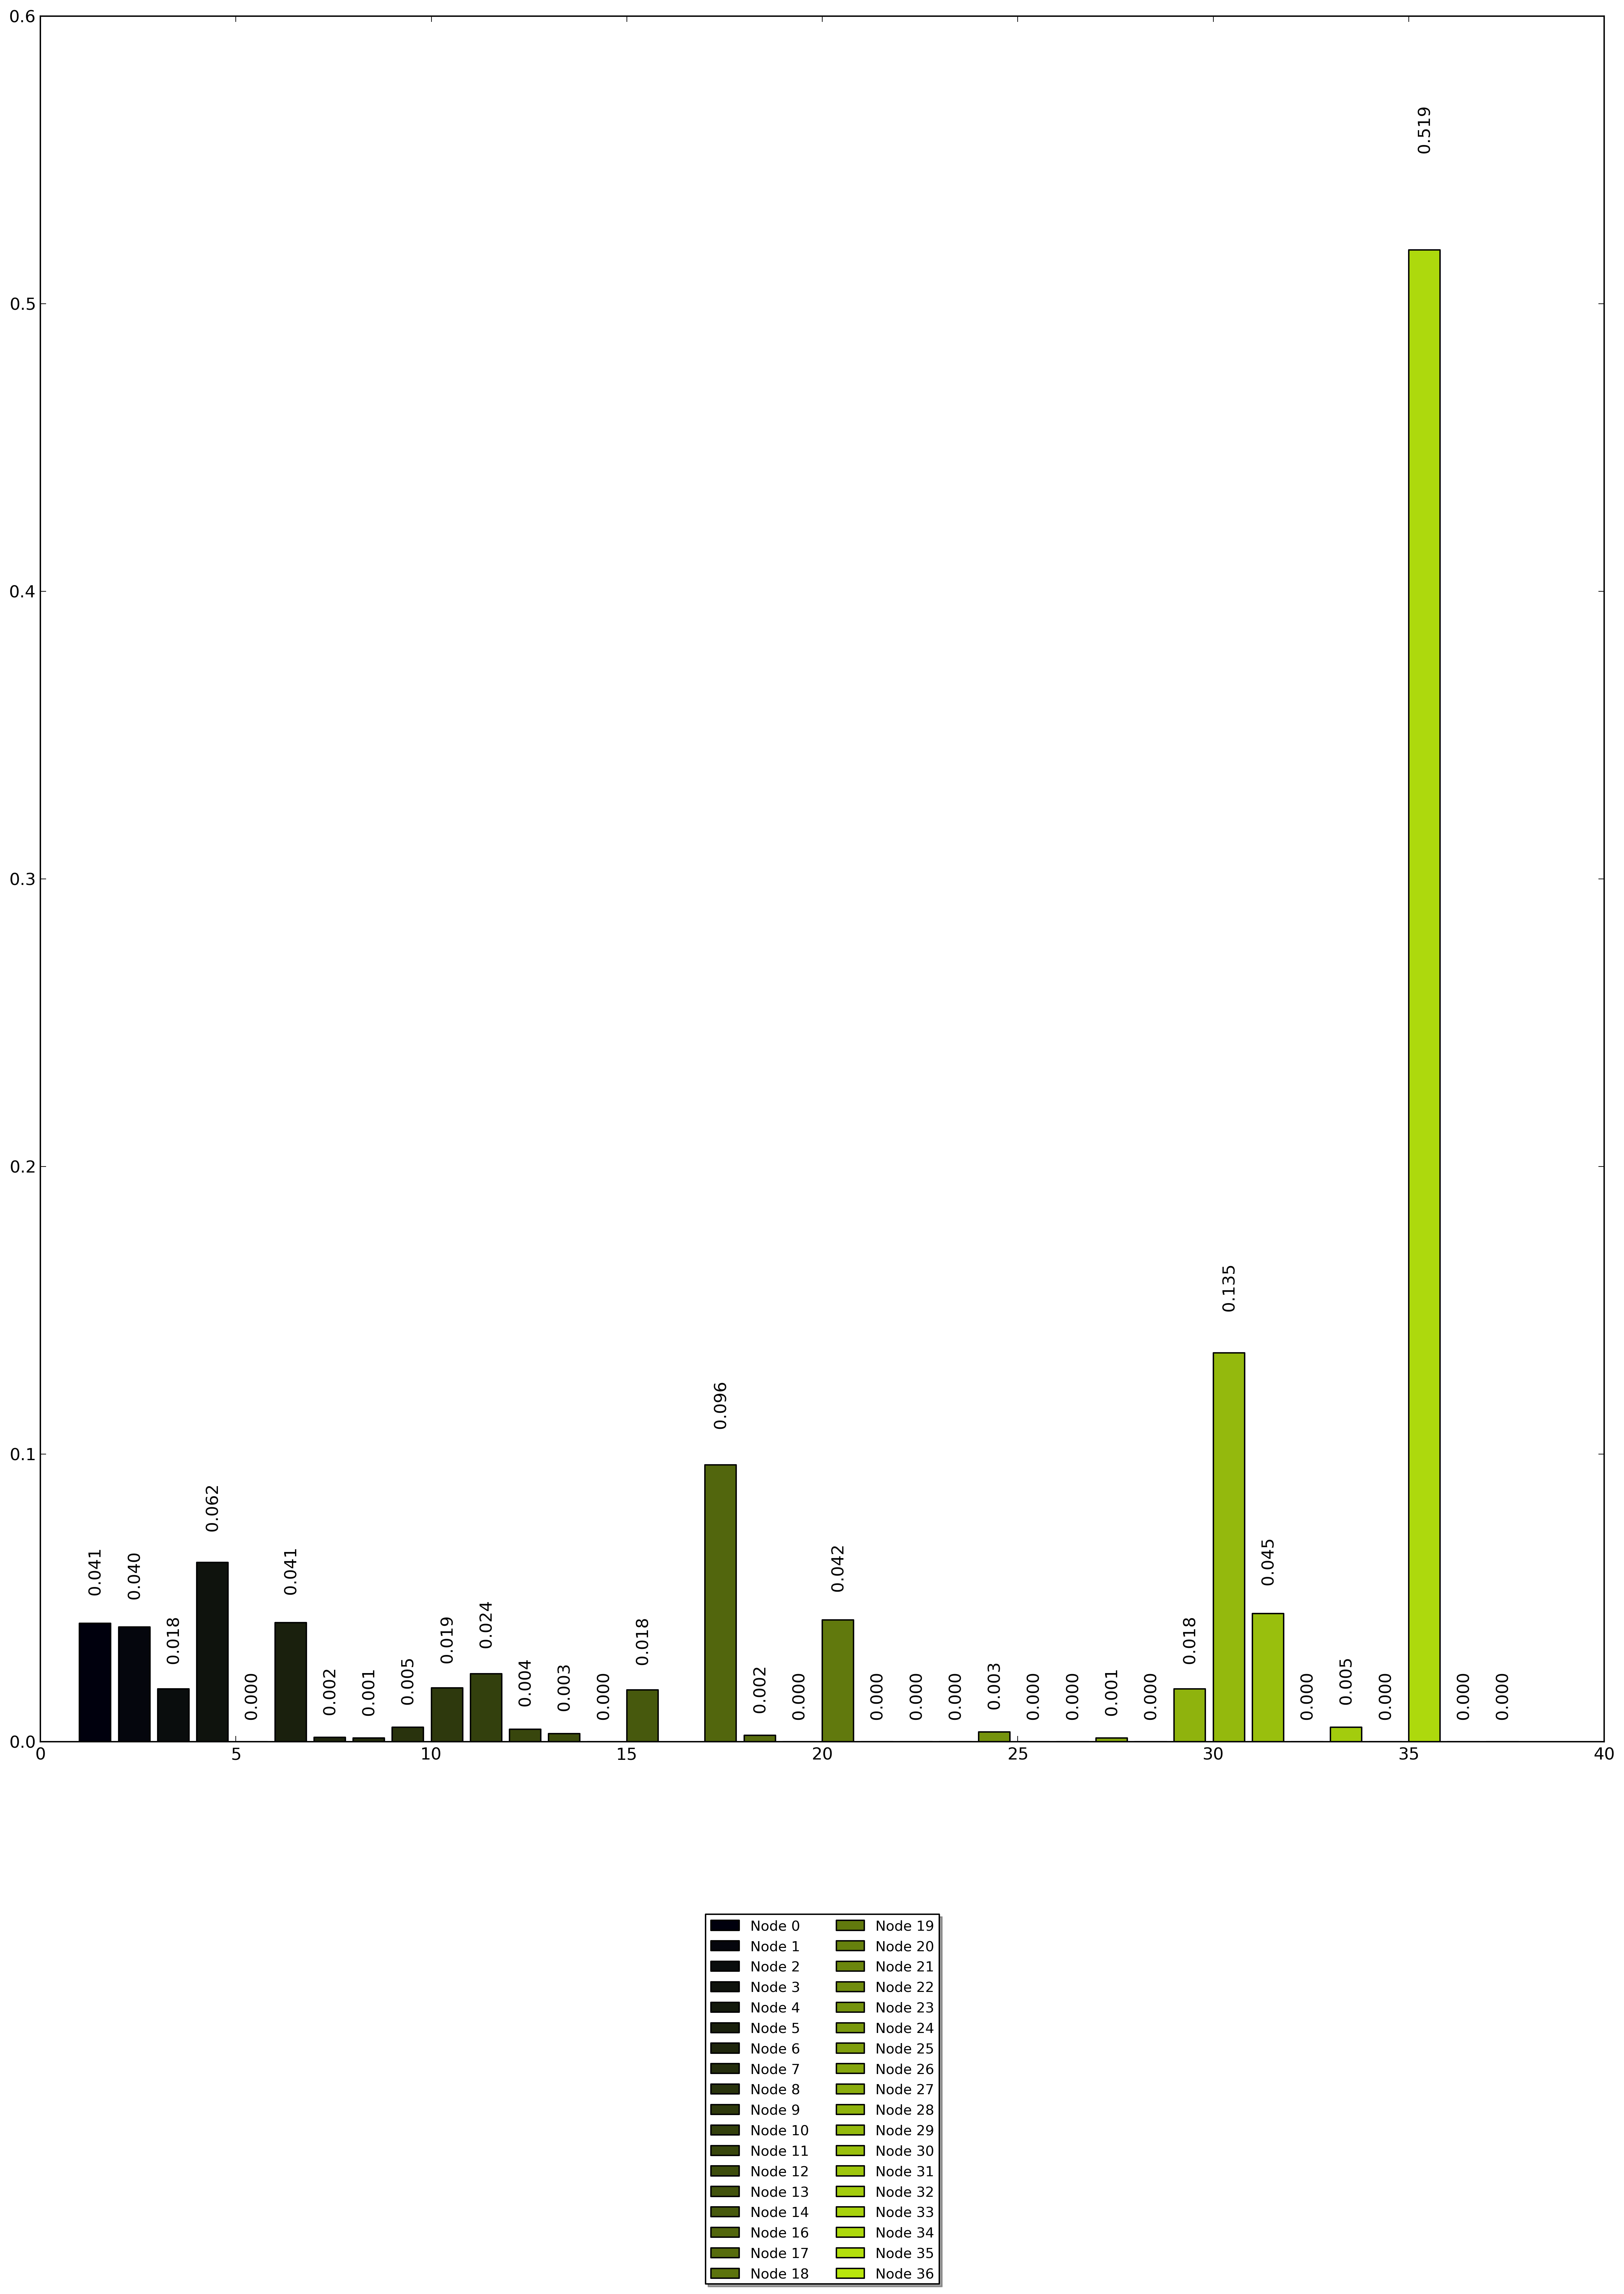
\includegraphics[scale=0.7]{resultsPL/Loss-rateALL.png}\\
  \caption{Bandwidth of all nodes.} \label{fig:loss-rate-plot}
\end{figure}
\end{center}


\section{GEO-Cloud Experiment Results}
\label{sec:geocloud-results}

